% Options for packages loaded elsewhere
\PassOptionsToPackage{unicode}{hyperref}
\PassOptionsToPackage{hyphens}{url}
\PassOptionsToPackage{dvipsnames,svgnames,x11names}{xcolor}
%
\documentclass[
  11pt,
]{article}

\usepackage{amsmath,amssymb}
\usepackage{iftex}
\ifPDFTeX
  \usepackage[T1]{fontenc}
  \usepackage[utf8]{inputenc}
  \usepackage{textcomp} % provide euro and other symbols
\else % if luatex or xetex
  \usepackage{unicode-math}
  \defaultfontfeatures{Scale=MatchLowercase}
  \defaultfontfeatures[\rmfamily]{Ligatures=TeX,Scale=1}
\fi
\usepackage{lmodern}
\ifPDFTeX\else  
    % xetex/luatex font selection
\fi
% Use upquote if available, for straight quotes in verbatim environments
\IfFileExists{upquote.sty}{\usepackage{upquote}}{}
\IfFileExists{microtype.sty}{% use microtype if available
  \usepackage[]{microtype}
  \UseMicrotypeSet[protrusion]{basicmath} % disable protrusion for tt fonts
}{}
\makeatletter
\@ifundefined{KOMAClassName}{% if non-KOMA class
  \IfFileExists{parskip.sty}{%
    \usepackage{parskip}
  }{% else
    \setlength{\parindent}{0pt}
    \setlength{\parskip}{6pt plus 2pt minus 1pt}}
}{% if KOMA class
  \KOMAoptions{parskip=half}}
\makeatother
\usepackage{xcolor}
\usepackage[margin=0.75in]{geometry}
\setlength{\emergencystretch}{3em} % prevent overfull lines
\setcounter{secnumdepth}{-\maxdimen} % remove section numbering
% Make \paragraph and \subparagraph free-standing
\ifx\paragraph\undefined\else
  \let\oldparagraph\paragraph
  \renewcommand{\paragraph}[1]{\oldparagraph{#1}\mbox{}}
\fi
\ifx\subparagraph\undefined\else
  \let\oldsubparagraph\subparagraph
  \renewcommand{\subparagraph}[1]{\oldsubparagraph{#1}\mbox{}}
\fi

\usepackage{color}
\usepackage{fancyvrb}
\newcommand{\VerbBar}{|}
\newcommand{\VERB}{\Verb[commandchars=\\\{\}]}
\DefineVerbatimEnvironment{Highlighting}{Verbatim}{commandchars=\\\{\}}
% Add ',fontsize=\small' for more characters per line
\usepackage{framed}
\definecolor{shadecolor}{RGB}{241,243,245}
\newenvironment{Shaded}{\begin{snugshade}}{\end{snugshade}}
\newcommand{\AlertTok}[1]{\textcolor[rgb]{0.68,0.00,0.00}{#1}}
\newcommand{\AnnotationTok}[1]{\textcolor[rgb]{0.37,0.37,0.37}{#1}}
\newcommand{\AttributeTok}[1]{\textcolor[rgb]{0.40,0.45,0.13}{#1}}
\newcommand{\BaseNTok}[1]{\textcolor[rgb]{0.68,0.00,0.00}{#1}}
\newcommand{\BuiltInTok}[1]{\textcolor[rgb]{0.00,0.23,0.31}{#1}}
\newcommand{\CharTok}[1]{\textcolor[rgb]{0.13,0.47,0.30}{#1}}
\newcommand{\CommentTok}[1]{\textcolor[rgb]{0.37,0.37,0.37}{#1}}
\newcommand{\CommentVarTok}[1]{\textcolor[rgb]{0.37,0.37,0.37}{\textit{#1}}}
\newcommand{\ConstantTok}[1]{\textcolor[rgb]{0.56,0.35,0.01}{#1}}
\newcommand{\ControlFlowTok}[1]{\textcolor[rgb]{0.00,0.23,0.31}{#1}}
\newcommand{\DataTypeTok}[1]{\textcolor[rgb]{0.68,0.00,0.00}{#1}}
\newcommand{\DecValTok}[1]{\textcolor[rgb]{0.68,0.00,0.00}{#1}}
\newcommand{\DocumentationTok}[1]{\textcolor[rgb]{0.37,0.37,0.37}{\textit{#1}}}
\newcommand{\ErrorTok}[1]{\textcolor[rgb]{0.68,0.00,0.00}{#1}}
\newcommand{\ExtensionTok}[1]{\textcolor[rgb]{0.00,0.23,0.31}{#1}}
\newcommand{\FloatTok}[1]{\textcolor[rgb]{0.68,0.00,0.00}{#1}}
\newcommand{\FunctionTok}[1]{\textcolor[rgb]{0.28,0.35,0.67}{#1}}
\newcommand{\ImportTok}[1]{\textcolor[rgb]{0.00,0.46,0.62}{#1}}
\newcommand{\InformationTok}[1]{\textcolor[rgb]{0.37,0.37,0.37}{#1}}
\newcommand{\KeywordTok}[1]{\textcolor[rgb]{0.00,0.23,0.31}{#1}}
\newcommand{\NormalTok}[1]{\textcolor[rgb]{0.00,0.23,0.31}{#1}}
\newcommand{\OperatorTok}[1]{\textcolor[rgb]{0.37,0.37,0.37}{#1}}
\newcommand{\OtherTok}[1]{\textcolor[rgb]{0.00,0.23,0.31}{#1}}
\newcommand{\PreprocessorTok}[1]{\textcolor[rgb]{0.68,0.00,0.00}{#1}}
\newcommand{\RegionMarkerTok}[1]{\textcolor[rgb]{0.00,0.23,0.31}{#1}}
\newcommand{\SpecialCharTok}[1]{\textcolor[rgb]{0.37,0.37,0.37}{#1}}
\newcommand{\SpecialStringTok}[1]{\textcolor[rgb]{0.13,0.47,0.30}{#1}}
\newcommand{\StringTok}[1]{\textcolor[rgb]{0.13,0.47,0.30}{#1}}
\newcommand{\VariableTok}[1]{\textcolor[rgb]{0.07,0.07,0.07}{#1}}
\newcommand{\VerbatimStringTok}[1]{\textcolor[rgb]{0.13,0.47,0.30}{#1}}
\newcommand{\WarningTok}[1]{\textcolor[rgb]{0.37,0.37,0.37}{\textit{#1}}}

\providecommand{\tightlist}{%
  \setlength{\itemsep}{0pt}\setlength{\parskip}{0pt}}\usepackage{longtable,booktabs,array}
\usepackage{calc} % for calculating minipage widths
% Correct order of tables after \paragraph or \subparagraph
\usepackage{etoolbox}
\makeatletter
\patchcmd\longtable{\par}{\if@noskipsec\mbox{}\fi\par}{}{}
\makeatother
% Allow footnotes in longtable head/foot
\IfFileExists{footnotehyper.sty}{\usepackage{footnotehyper}}{\usepackage{footnote}}
\makesavenoteenv{longtable}
\usepackage{graphicx}
\makeatletter
\def\maxwidth{\ifdim\Gin@nat@width>\linewidth\linewidth\else\Gin@nat@width\fi}
\def\maxheight{\ifdim\Gin@nat@height>\textheight\textheight\else\Gin@nat@height\fi}
\makeatother
% Scale images if necessary, so that they will not overflow the page
% margins by default, and it is still possible to overwrite the defaults
% using explicit options in \includegraphics[width, height, ...]{}
\setkeys{Gin}{width=\maxwidth,height=\maxheight,keepaspectratio}
% Set default figure placement to htbp
\makeatletter
\def\fps@figure{htbp}
\makeatother

\usepackage{fvextra}
\DefineVerbatimEnvironment{Highlighting}{Verbatim}{breaklines,commandchars=\\\{\}}
\DefineVerbatimEnvironment{OutputCode}{Verbatim}{breaklines,commandchars=\\\{\}}
\fvset{breaksymbolleft={}, breakindent=1em}
\makeatletter
\@ifpackageloaded{caption}{}{\usepackage{caption}}
\AtBeginDocument{%
\ifdefined\contentsname
  \renewcommand*\contentsname{Table of contents}
\else
  \newcommand\contentsname{Table of contents}
\fi
\ifdefined\listfigurename
  \renewcommand*\listfigurename{List of Figures}
\else
  \newcommand\listfigurename{List of Figures}
\fi
\ifdefined\listtablename
  \renewcommand*\listtablename{List of Tables}
\else
  \newcommand\listtablename{List of Tables}
\fi
\ifdefined\figurename
  \renewcommand*\figurename{Figure}
\else
  \newcommand\figurename{Figure}
\fi
\ifdefined\tablename
  \renewcommand*\tablename{Table}
\else
  \newcommand\tablename{Table}
\fi
}
\@ifpackageloaded{float}{}{\usepackage{float}}
\floatstyle{ruled}
\@ifundefined{c@chapter}{\newfloat{codelisting}{h}{lop}}{\newfloat{codelisting}{h}{lop}[chapter]}
\floatname{codelisting}{Listing}
\newcommand*\listoflistings{\listof{codelisting}{List of Listings}}
\makeatother
\makeatletter
\makeatother
\makeatletter
\@ifpackageloaded{caption}{}{\usepackage{caption}}
\@ifpackageloaded{subcaption}{}{\usepackage{subcaption}}
\makeatother
\ifLuaTeX
  \usepackage{selnolig}  % disable illegal ligatures
\fi
\usepackage{bookmark}

\IfFileExists{xurl.sty}{\usepackage{xurl}}{} % add URL line breaks if available
\urlstyle{same} % disable monospaced font for URLs
\hypersetup{
  pdftitle={Homework 3},
  pdfauthor={Nick Climaco},
  colorlinks=true,
  linkcolor={blue},
  filecolor={Maroon},
  citecolor={Blue},
  urlcolor={Blue},
  pdfcreator={LaTeX via pandoc}}

\title{Homework 3}
\author{Nick Climaco}
\date{February 16, 2024}

\begin{document}
\maketitle

\RecustomVerbatimEnvironment{verbatim}{Verbatim}{
  showspaces = false,
  showtabs = false,
  breaksymbolleft={},
  breaklines
}

\renewcommand*\contentsname{Table of contents}
{
\hypersetup{linkcolor=}
\setcounter{tocdepth}{3}
\tableofcontents
}
\newpage

\section{Chapter 5: The Forecaster's
Toolbox}\label{chapter-5-the-forecasters-toolbox}

\begin{Shaded}
\begin{Highlighting}[]
\CommentTok{\# data wrangling }
\ImportTok{import}\NormalTok{ pandas }\ImportTok{as}\NormalTok{ pd }
\ImportTok{import}\NormalTok{ numpy }\ImportTok{as}\NormalTok{ np}

\CommentTok{\# data visuals}
\ImportTok{import}\NormalTok{ matplotlib.pyplot }\ImportTok{as}\NormalTok{ plt }
\ImportTok{import}\NormalTok{ seaborn }\ImportTok{as}\NormalTok{ sns}

\CommentTok{\# timeseries analysis}
\ImportTok{from}\NormalTok{ darts }\ImportTok{import}\NormalTok{ TimeSeries}

\CommentTok{\# ts decomposition}
\ImportTok{from}\NormalTok{ statsmodels.tsa.seasonal }\ImportTok{import}\NormalTok{ STL}
\ImportTok{from}\NormalTok{ statsmodels.tsa.seasonal }\ImportTok{import}\NormalTok{ seasonal\_decompose}

\CommentTok{\# forecasting method}
\ImportTok{from}\NormalTok{ darts.models }\ImportTok{import}\NormalTok{ NaiveMean}
\ImportTok{from}\NormalTok{ darts.models }\ImportTok{import}\NormalTok{ NaiveSeasonal }\CommentTok{\# K=1 for last value, K=4 for quarterly data}
\ImportTok{from}\NormalTok{ darts.models }\ImportTok{import}\NormalTok{ NaiveDrift}
\end{Highlighting}
\end{Shaded}

\begin{verbatim}
c:\Users\nickc\DataScience\ds_env\Lib\site-packages\statsforecast\core.py:26: TqdmWarning: IProgress not found. Please update jupyter and ipywidgets. See https://ipywidgets.readthedocs.io/en/stable/user_install.html
  from tqdm.autonotebook import tqdm
\end{verbatim}

Resource:

\begin{itemize}
\tightlist
\item
  \href{https://unit8co.github.io/darts/quickstart/00-quickstart.html}{Darts
  Documentation}
\end{itemize}

\subsection{Exercise 1}\label{exercise-1}

Produce forecasts for the following series using whichever of NAIVE(y),
SNAIVE(y) or RW(y \textasciitilde{} drift()) is more appropriate in each
case:

\begin{itemize}
\item
  Australian Population (global\_economy)
\item
  Bricks (aus\_production)
\item
  NSW Lambs (aus\_livestock)
\item
  Household wealth (hh\_budget).
\item
  Australian takeaway food turnover (aus\_retail).
\end{itemize}

\begin{Shaded}
\begin{Highlighting}[]
\CommentTok{\# reading in the data}
\NormalTok{df\_global\_economy }\OperatorTok{=}\NormalTok{ pd.read\_csv(}\StringTok{"../rdata/global\_economy.csv"}\NormalTok{, parse\_dates}\OperatorTok{=}\NormalTok{[}\StringTok{\textquotesingle{}Year\textquotesingle{}}\NormalTok{])}
\NormalTok{df\_production}\OperatorTok{=}\NormalTok{ pd.read\_csv(}\StringTok{"../rdata/aus\_production.csv"}\NormalTok{, parse\_dates}\OperatorTok{=}\NormalTok{[}\StringTok{\textquotesingle{}Quarter\textquotesingle{}}\NormalTok{])}
\NormalTok{df\_livestock }\OperatorTok{=}\NormalTok{ pd.read\_csv(}\StringTok{"../rdata/aus\_livestock.csv"}\NormalTok{, parse\_dates}\OperatorTok{=}\NormalTok{[}\StringTok{\textquotesingle{}Month\textquotesingle{}}\NormalTok{])}
\NormalTok{df\_budget }\OperatorTok{=}\NormalTok{ pd.read\_csv(}\StringTok{"../rdata/hh\_budget.csv"}\NormalTok{, parse\_dates}\OperatorTok{=}\NormalTok{[}\StringTok{\textquotesingle{}Year\textquotesingle{}}\NormalTok{])}
\NormalTok{df\_retail }\OperatorTok{=}\NormalTok{ pd.read\_csv(}\StringTok{"../rdata/aus\_retail.csv"}\NormalTok{,parse\_dates}\OperatorTok{=}\NormalTok{[}\StringTok{\textquotesingle{}Month\textquotesingle{}}\NormalTok{])}
\end{Highlighting}
\end{Shaded}

\subsubsection{\texorpdfstring{Australian Population from
\texttt{global\_economy}}{Australian Population from global\_economy}}\label{australian-population-from-global_economy}

\begin{Shaded}
\begin{Highlighting}[]
\CommentTok{\# filter australia}
\NormalTok{df\_aus }\OperatorTok{=}\NormalTok{ df\_global\_economy.query(}\StringTok{\textquotesingle{}Country == "Australia"\textquotesingle{}}\NormalTok{)}
\end{Highlighting}
\end{Shaded}

\begin{Shaded}
\begin{Highlighting}[]
\CommentTok{\# plot australian timeseries pop}
\NormalTok{df\_aus\_pop }\OperatorTok{=}\NormalTok{ df\_aus[[}\StringTok{\textquotesingle{}Year\textquotesingle{}}\NormalTok{, }\StringTok{\textquotesingle{}Population\textquotesingle{}}\NormalTok{]]}
\NormalTok{df\_aus\_pop.set\_index(}\StringTok{\textquotesingle{}Year\textquotesingle{}}\NormalTok{, inplace}\OperatorTok{=}\VariableTok{True}\NormalTok{)}
\NormalTok{df\_aus\_pop.plot()}
\end{Highlighting}
\end{Shaded}

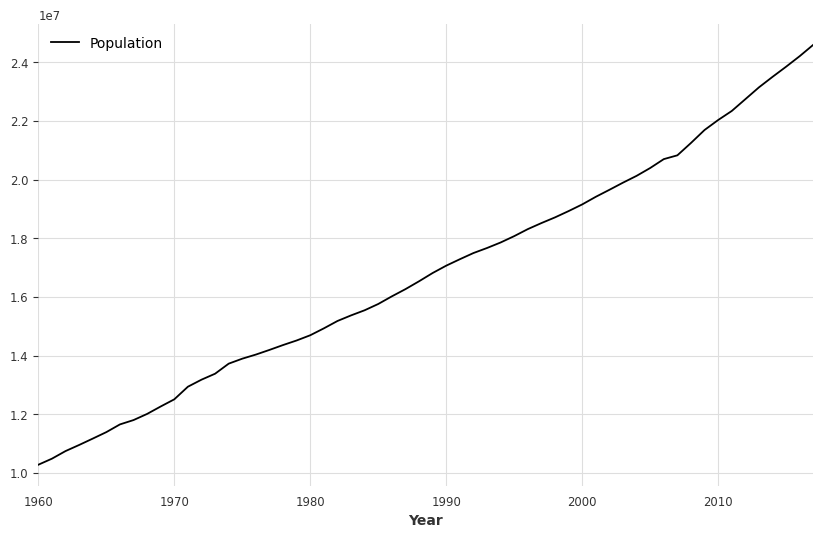
\includegraphics{hw3_files/figure-pdf/cell-6-output-1.png}

The Australian Populatiion has near perfect linear growth from the 1960
to 2020. Before, choosing which forecasting method to go with. I would
like to see the decomposition of this time series just to make sure that
my initial observation of no seasonality is correct.

\begin{Shaded}
\begin{Highlighting}[]
\CommentTok{\# decompose this ts }
\NormalTok{decomposition }\OperatorTok{=}\NormalTok{ seasonal\_decompose(df\_aus\_pop.Population, period }\OperatorTok{=} \DecValTok{1}\NormalTok{, model}\OperatorTok{=}\StringTok{"multiplicative"}\NormalTok{)}

\NormalTok{fig, (ax1, ax2, ax3, ax4) }\OperatorTok{=}\NormalTok{ plt.subplots(}\DecValTok{4}\NormalTok{, }\DecValTok{1}\NormalTok{, figsize}\OperatorTok{=}\NormalTok{(}\DecValTok{10}\NormalTok{, }\DecValTok{8}\NormalTok{))}

\NormalTok{ax1.plot(decomposition.observed)}
\NormalTok{ax1.set\_title(}\StringTok{\textquotesingle{}Observed\textquotesingle{}}\NormalTok{)}

\NormalTok{ax2.plot(decomposition.trend)}
\NormalTok{ax2.set\_title(}\StringTok{\textquotesingle{}Trend\textquotesingle{}}\NormalTok{)}

\NormalTok{ax3.plot(decomposition.seasonal)}
\NormalTok{ax3.set\_title(}\StringTok{\textquotesingle{}Seasonal\textquotesingle{}}\NormalTok{)}

\NormalTok{ax4.plot(decomposition.resid, linestyle }\OperatorTok{=} \StringTok{"dotted"}\NormalTok{, markersize }\OperatorTok{=} \DecValTok{10}\NormalTok{)}
\NormalTok{ax4.set\_title(}\StringTok{\textquotesingle{}Residual\textquotesingle{}}\NormalTok{)}

\NormalTok{plt.tight\_layout()}
\NormalTok{plt.show()}
\end{Highlighting}
\end{Shaded}

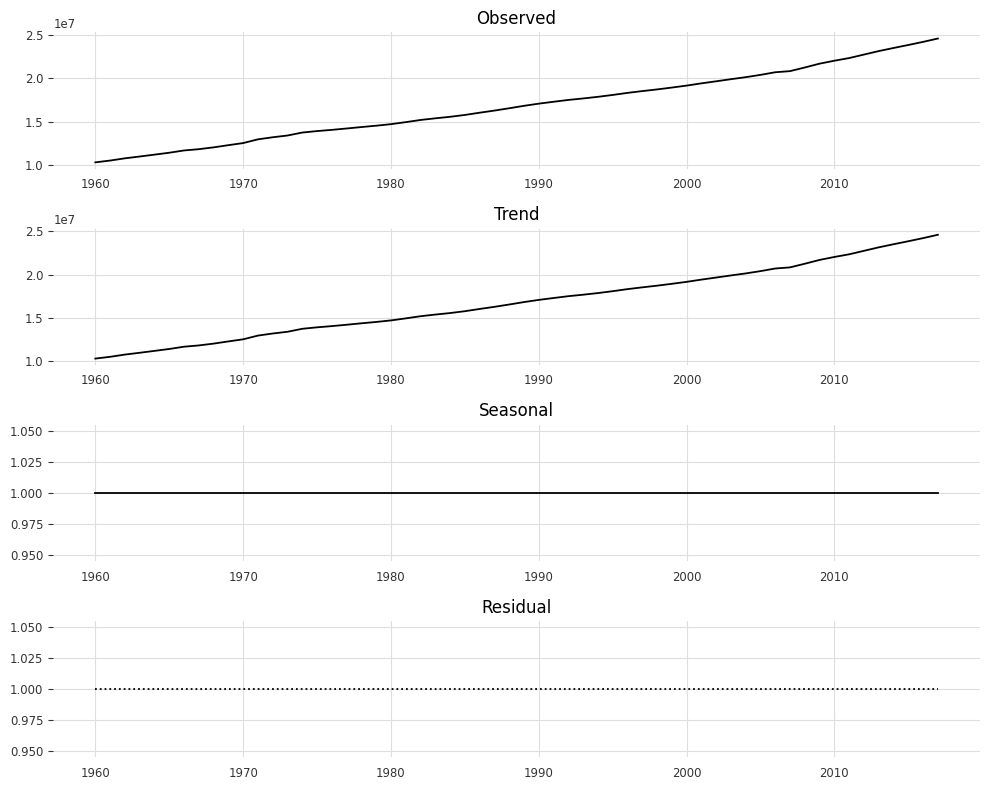
\includegraphics{hw3_files/figure-pdf/cell-7-output-1.png}

The trend line captures almost all of the observed data indicated that
the seasonal component is constant at a value of 1. Thus, I believe that
using the Drift method would be the most appropriate for this timeseries
since it exhibits no seasonality and a overal upward trend. Wherein our
forecast cast would be the average change seen in the data.

\begin{Shaded}
\begin{Highlighting}[]
\CommentTok{\# convert df to ts }
\NormalTok{series }\OperatorTok{=}\NormalTok{ TimeSeries.from\_dataframe(df\_aus,}\StringTok{\textquotesingle{}Year\textquotesingle{}}\NormalTok{, }\StringTok{\textquotesingle{}Population\textquotesingle{}}\NormalTok{)}
\end{Highlighting}
\end{Shaded}

\begin{Shaded}
\begin{Highlighting}[]
\NormalTok{drift }\OperatorTok{=}\NormalTok{ NaiveDrift()}

\NormalTok{drift.fit(series)}

\NormalTok{forecast }\OperatorTok{=}\NormalTok{ drift.predict(}\DecValTok{10}\NormalTok{) }\CommentTok{\# 10 timesteps}
\NormalTok{series.plot()}
\NormalTok{forecast.plot(label}\OperatorTok{=}\StringTok{\textquotesingle{}Drift Forecast\textquotesingle{}}\NormalTok{, low\_quantile }\OperatorTok{=} \FloatTok{0.05}\NormalTok{, high\_quantile}\OperatorTok{=}\FloatTok{0.95}\NormalTok{)}
\NormalTok{plt.legend()}
\end{Highlighting}
\end{Shaded}

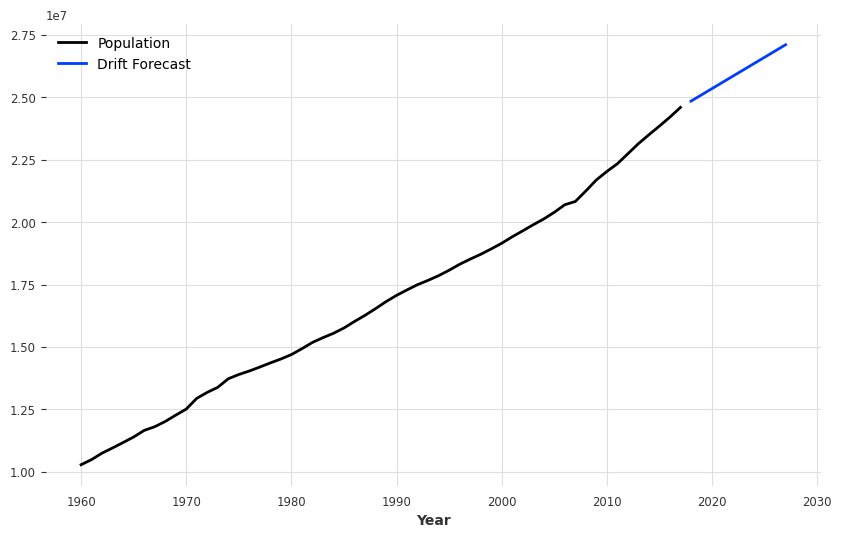
\includegraphics{hw3_files/figure-pdf/cell-9-output-1.png}

From the eye test, we observe that the Drift forecast is in-line with
the data. It reasonable to agree with the forecast since the timeseries
demonstrates an linear growth in population.

\subsubsection{\texorpdfstring{Bricks from
\texttt{aus\_production}}{Bricks from aus\_production}}\label{bricks-from-aus_production}

\begin{Shaded}
\begin{Highlighting}[]
\NormalTok{df\_bricks }\OperatorTok{=}\NormalTok{ df\_production[[}\StringTok{\textquotesingle{}Quarter\textquotesingle{}}\NormalTok{, }\StringTok{\textquotesingle{}Bricks\textquotesingle{}}\NormalTok{]]}
\end{Highlighting}
\end{Shaded}

\begin{Shaded}
\begin{Highlighting}[]
\NormalTok{df\_bricks.set\_index(}\StringTok{\textquotesingle{}Quarter\textquotesingle{}}\NormalTok{).plot()}
\end{Highlighting}
\end{Shaded}

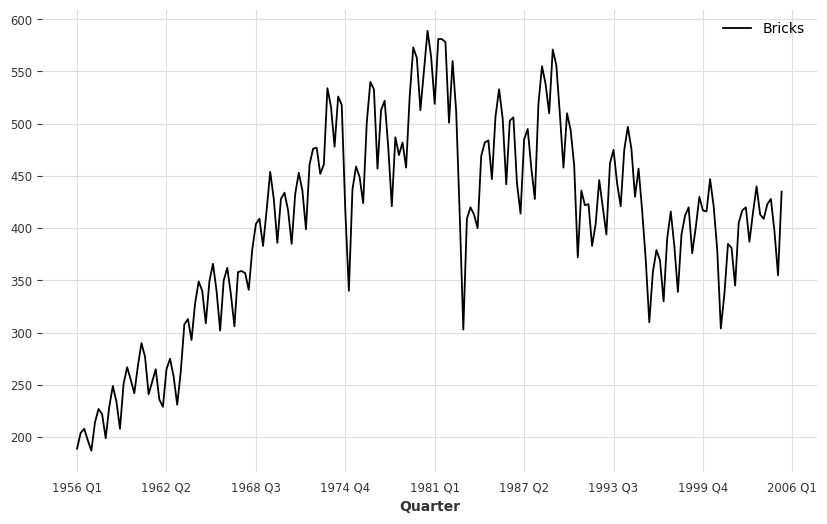
\includegraphics{hw3_files/figure-pdf/cell-11-output-1.png}

\begin{Shaded}
\begin{Highlighting}[]
\NormalTok{bricks\_plot }\OperatorTok{=}\NormalTok{ df\_bricks.set\_index(}\StringTok{\textquotesingle{}Quarter\textquotesingle{}}\NormalTok{)}
\NormalTok{bricks\_plot[}\StringTok{\textquotesingle{}Bricks\textquotesingle{}}\NormalTok{] }\OperatorTok{=}\NormalTok{ bricks\_plot[}\StringTok{\textquotesingle{}Bricks\textquotesingle{}}\NormalTok{].ffill()}

\NormalTok{decom }\OperatorTok{=}\NormalTok{ STL(bricks\_plot[}\StringTok{\textquotesingle{}Bricks\textquotesingle{}}\NormalTok{].values, period }\OperatorTok{=} \DecValTok{4}\NormalTok{).fit()}
\NormalTok{decom.plot()}
\NormalTok{plt.show()}
\end{Highlighting}
\end{Shaded}

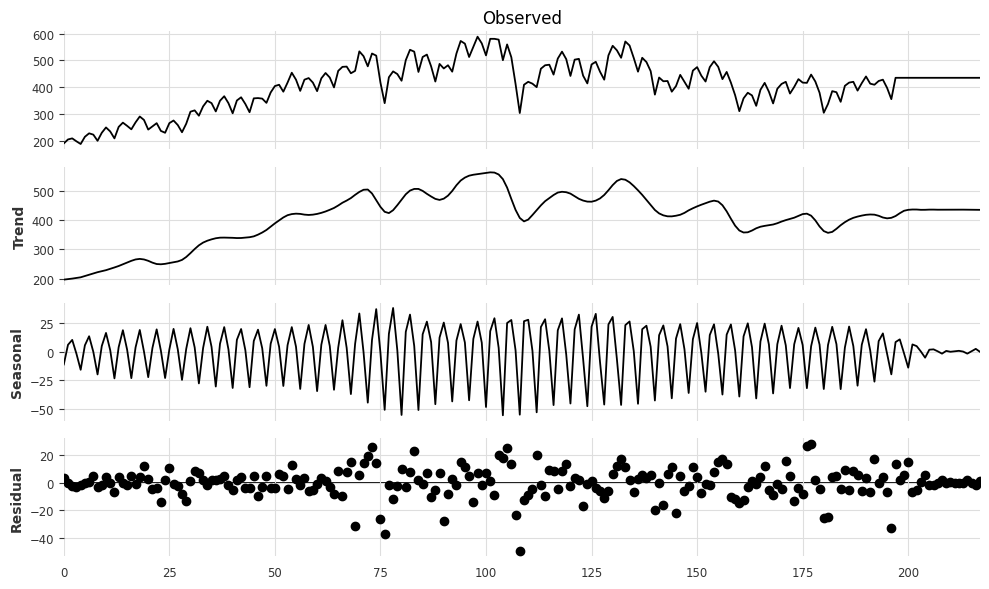
\includegraphics{hw3_files/figure-pdf/cell-12-output-1.png}

We see a high frequency of the seasonality component while it is unclear
whether the trend line is increasing or decreasing. Thus, we believe
that using the seasonal naive would be best for forecasting this
particular time series.

\begin{Shaded}
\begin{Highlighting}[]
\NormalTok{df\_bricks }\OperatorTok{=}\NormalTok{ df\_bricks.dropna() }\CommentTok{\# missing a data at the tail() }

\CommentTok{\# format datetime to accomodate the input for darts library}
\NormalTok{df\_bricks[}\StringTok{\textquotesingle{}Quarter\textquotesingle{}}\NormalTok{] }\OperatorTok{=}\NormalTok{ pd.to\_datetime(df\_bricks[}\StringTok{\textquotesingle{}Quarter\textquotesingle{}}\NormalTok{].astype(}\BuiltInTok{str}\NormalTok{), }\BuiltInTok{format}\OperatorTok{=}\StringTok{\textquotesingle{}\%Y Q\%m\textquotesingle{}}\NormalTok{)}

\NormalTok{df\_bricks.set\_index(}\StringTok{\textquotesingle{}Quarter\textquotesingle{}}\NormalTok{)}
\end{Highlighting}
\end{Shaded}

\begin{longtable}[]{@{}ll@{}}
\toprule\noalign{}
& Bricks \\
Quarter & \\
\midrule\noalign{}
\endhead
\bottomrule\noalign{}
\endlastfoot
1956-01-01 & 189.0 \\
1956-02-01 & 204.0 \\
1956-03-01 & 208.0 \\
1956-04-01 & 197.0 \\
1957-01-01 & 187.0 \\
... & ... \\
2004-02-01 & 423.0 \\
2004-03-01 & 428.0 \\
2004-04-01 & 397.0 \\
2005-01-01 & 355.0 \\
2005-02-01 & 435.0 \\
\end{longtable}

\begin{Shaded}
\begin{Highlighting}[]
\CommentTok{\# remove time col since it is set as the index}
\NormalTok{series }\OperatorTok{=}\NormalTok{ TimeSeries.from\_dataframe(df\_bricks, value\_cols}\OperatorTok{=}\StringTok{\textquotesingle{}Bricks\textquotesingle{}}\NormalTok{, fill\_missing\_dates}\OperatorTok{=}\VariableTok{True}\NormalTok{)}

\NormalTok{seasonal }\OperatorTok{=}\NormalTok{ NaiveSeasonal(K}\OperatorTok{=}\DecValTok{4}\NormalTok{) }\CommentTok{\# K=4 for quarterly data}

\NormalTok{seasonal.fit(series)}

\NormalTok{forecast }\OperatorTok{=}\NormalTok{ seasonal.predict(}\DecValTok{16}\NormalTok{)}

\NormalTok{series.plot()}
\NormalTok{forecast.plot(label}\OperatorTok{=}\StringTok{\textquotesingle{}Naive Seasonal Forecast\textquotesingle{}}\NormalTok{)}
\NormalTok{plt.legend()}
\end{Highlighting}
\end{Shaded}

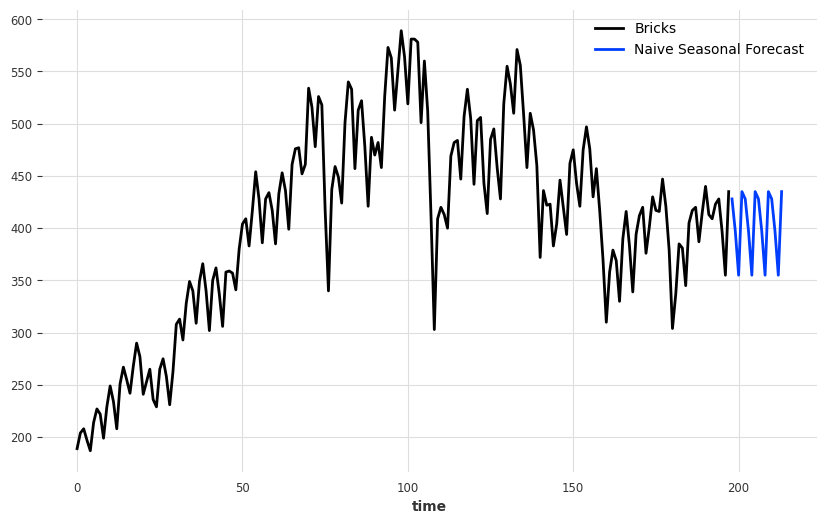
\includegraphics{hw3_files/figure-pdf/cell-14-output-1.png}

\subsubsection{\texorpdfstring{NSW Lambs from
\texttt{aus\_livestock}}{NSW Lambs from aus\_livestock}}\label{nsw-lambs-from-aus_livestock}

\begin{Shaded}
\begin{Highlighting}[]
\NormalTok{display(df\_livestock.State.unique())}
\NormalTok{display(df\_livestock.Animal.unique())}
\end{Highlighting}
\end{Shaded}

\begin{verbatim}
array(['Australian Capital Territory', 'New South Wales',
       'Northern Territory', 'Queensland', 'South Australia', 'Tasmania',
       'Victoria', 'Western Australia'], dtype=object)
\end{verbatim}

\begin{verbatim}
array(['Bulls, bullocks and steers', 'Calves', 'Cattle (excl. calves)',
       'Cows and heifers', 'Lambs', 'Pigs', 'Sheep'], dtype=object)
\end{verbatim}

Assuming NSW means New South Wales. So, we need to filter
\texttt{df\_livestock} of sheep from New South Wales.

\begin{Shaded}
\begin{Highlighting}[]
\NormalTok{df\_sheep }\OperatorTok{=}\NormalTok{ df\_livestock.query(}\StringTok{\textquotesingle{}Animal == "Sheep" \& State == "New South Wales"\textquotesingle{}}\NormalTok{)}
\NormalTok{df\_sheep}
\end{Highlighting}
\end{Shaded}

\begin{longtable}[]{@{}llllll@{}}
\toprule\noalign{}
& Unnamed: 0 & Month & Animal & State & Count \\
\midrule\noalign{}
\endhead
\bottomrule\noalign{}
\endlastfoot
25458 & 25459 & 1972-07-01 & Sheep & New South Wales & 669400.0 \\
25459 & 25460 & 1972-08-01 & Sheep & New South Wales & 581100.0 \\
25460 & 25461 & 1972-09-01 & Sheep & New South Wales & 468100.0 \\
25461 & 25462 & 1972-10-01 & Sheep & New South Wales & 515300.0 \\
25462 & 25463 & 1972-11-01 & Sheep & New South Wales & 564500.0 \\
... & ... & ... & ... & ... & ... \\
26011 & 26012 & 2018-08-01 & Sheep & New South Wales & 245900.0 \\
26012 & 26013 & 2018-09-01 & Sheep & New South Wales & 236800.0 \\
26013 & 26014 & 2018-10-01 & Sheep & New South Wales & 277200.0 \\
26014 & 26015 & 2018-11-01 & Sheep & New South Wales & 263600.0 \\
26015 & 26016 & 2018-12-01 & Sheep & New South Wales & 212300.0 \\
\end{longtable}

Next, we want to see the timeseries.

\begin{Shaded}
\begin{Highlighting}[]
\NormalTok{df\_sheep[[}\StringTok{\textquotesingle{}Month\textquotesingle{}}\NormalTok{, }\StringTok{\textquotesingle{}Count\textquotesingle{}}\NormalTok{]].set\_index([}\StringTok{\textquotesingle{}Month\textquotesingle{}}\NormalTok{]).plot()}
\end{Highlighting}
\end{Shaded}

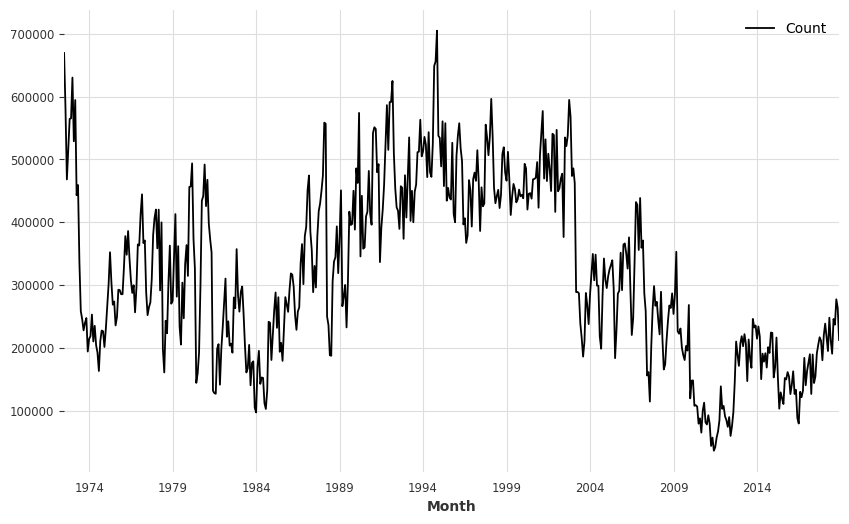
\includegraphics{hw3_files/figure-pdf/cell-17-output-1.png}

\begin{Shaded}
\begin{Highlighting}[]
\NormalTok{sheep }\OperatorTok{=}\NormalTok{ df\_sheep.set\_index(}\StringTok{\textquotesingle{}Month\textquotesingle{}}\NormalTok{)}
\NormalTok{decomposition }\OperatorTok{=}\NormalTok{ STL(sheep[}\StringTok{\textquotesingle{}Count\textquotesingle{}}\NormalTok{]).fit()}
\NormalTok{decomposition.plot()}
\NormalTok{plt.show()}
\end{Highlighting}
\end{Shaded}

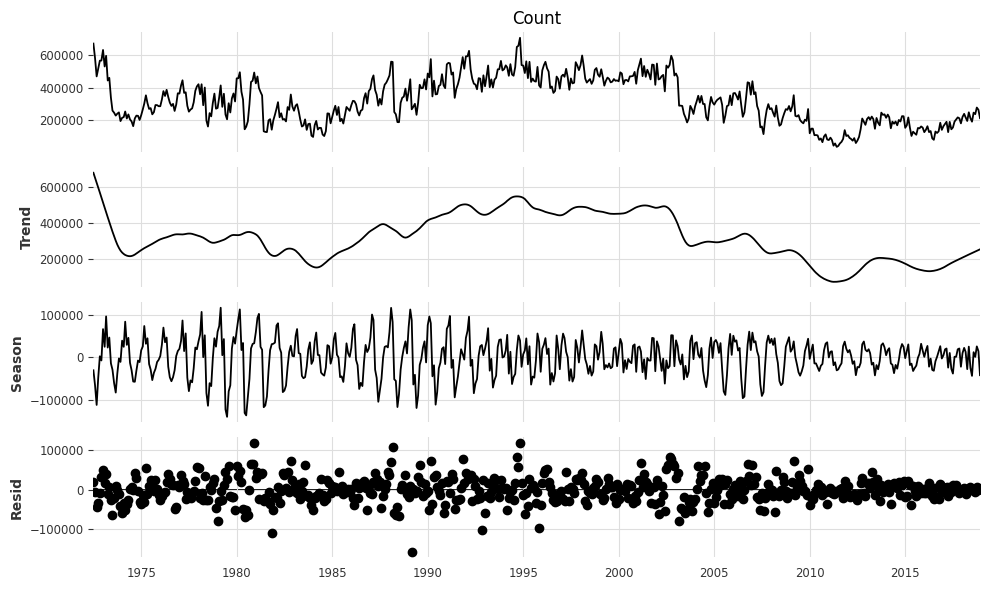
\includegraphics{hw3_files/figure-pdf/cell-18-output-1.png}

We see that this time seres has no clear trend and inconsistent
seasonality component which suggest that we use the Mean Naive method.

\begin{Shaded}
\begin{Highlighting}[]
\NormalTok{series }\OperatorTok{=}\NormalTok{ TimeSeries.from\_dataframe(df\_sheep, }\StringTok{\textquotesingle{}Month\textquotesingle{}}\NormalTok{, }\StringTok{\textquotesingle{}Count\textquotesingle{}}\NormalTok{)}

\NormalTok{model }\OperatorTok{=}\NormalTok{ NaiveMean() }
\NormalTok{model.fit(series)}
\NormalTok{forecast }\OperatorTok{=}\NormalTok{ model.predict(}\DecValTok{30}\NormalTok{) }\CommentTok{\# 30 timesteps in the future in this case 30 months}

\NormalTok{series.plot()}
\NormalTok{forecast.plot(label }\OperatorTok{=} \StringTok{\textquotesingle{}Naive Mean Forecast\textquotesingle{}}\NormalTok{)}
\NormalTok{plt.legend()}
\end{Highlighting}
\end{Shaded}

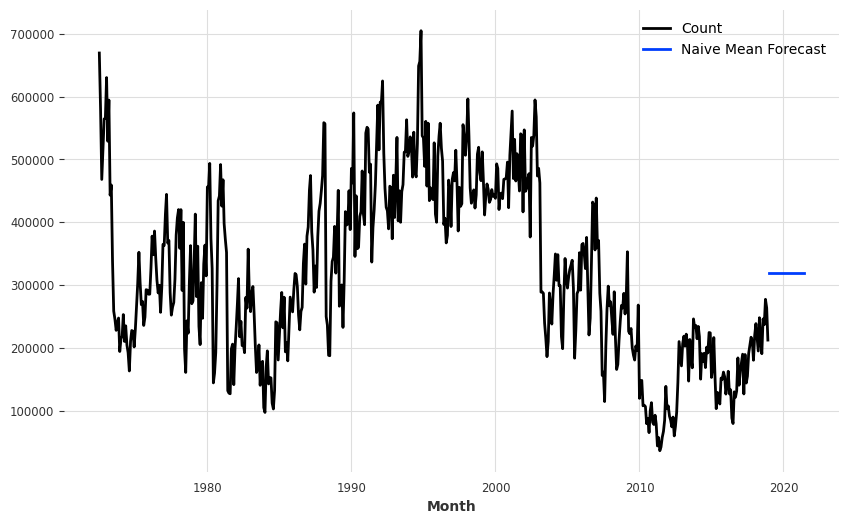
\includegraphics{hw3_files/figure-pdf/cell-19-output-1.png}

\subsubsection{\texorpdfstring{Household Wealth from
\texttt{hh\_budget}}{Household Wealth from hh\_budget}}\label{household-wealth-from-hh_budget}

Let us see which columns and constrains we need to filter. We will need
the \texttt{Year}, \texttt{Country} and \texttt{Wealth} columns.

\begin{Shaded}
\begin{Highlighting}[]
\NormalTok{df\_wealth }\OperatorTok{=}\NormalTok{ df\_budget[[}\StringTok{\textquotesingle{}Year\textquotesingle{}}\NormalTok{, }\StringTok{\textquotesingle{}Country\textquotesingle{}}\NormalTok{, }\StringTok{\textquotesingle{}Wealth\textquotesingle{}}\NormalTok{]]}
\NormalTok{df\_wealth}
\end{Highlighting}
\end{Shaded}

\begin{longtable}[]{@{}llll@{}}
\toprule\noalign{}
& Year & Country & Wealth \\
\midrule\noalign{}
\endhead
\bottomrule\noalign{}
\endlastfoot
0 & 1995-01-01 & Australia & 314.9344 \\
1 & 1996-01-01 & Australia & 314.5559 \\
2 & 1997-01-01 & Australia & 323.2357 \\
3 & 1998-01-01 & Australia & 339.3139 \\
4 & 1999-01-01 & Australia & 354.4382 \\
... & ... & ... & ... \\
83 & 2012-01-01 & USA & 514.4276 \\
84 & 2013-01-01 & USA & 592.3568 \\
85 & 2014-01-01 & USA & 596.4713 \\
86 & 2015-01-01 & USA & 588.1454 \\
87 & 2016-01-01 & USA & 609.2657 \\
\end{longtable}

So, we have annual data for wealth of four different countries. Based on
the prior exercise, we can assume that we want the Australian data.

\begin{Shaded}
\begin{Highlighting}[]
\NormalTok{wealth }\OperatorTok{=}\NormalTok{ df\_wealth}
\NormalTok{wealth }\OperatorTok{=}\NormalTok{ wealth.set\_index([}\StringTok{\textquotesingle{}Year\textquotesingle{}}\NormalTok{])}

\NormalTok{wealth.groupby(}\StringTok{\textquotesingle{}Country\textquotesingle{}}\NormalTok{)[}\StringTok{\textquotesingle{}Wealth\textquotesingle{}}\NormalTok{].plot()}
\NormalTok{plt.legend()}
\end{Highlighting}
\end{Shaded}

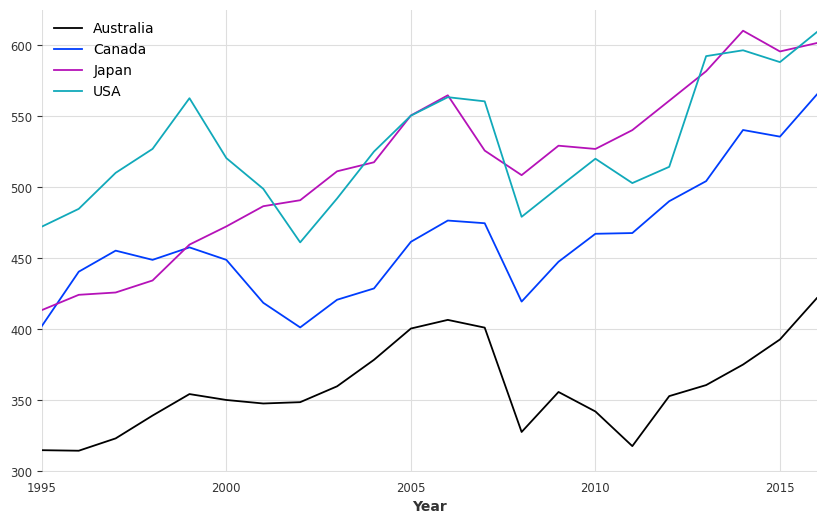
\includegraphics{hw3_files/figure-pdf/cell-21-output-1.png}

\begin{Shaded}
\begin{Highlighting}[]
\NormalTok{aus\_wealth }\OperatorTok{=}\NormalTok{ wealth.query(}\StringTok{\textquotesingle{}Country == "Australia"\textquotesingle{}}\NormalTok{)}
\end{Highlighting}
\end{Shaded}

\begin{Shaded}
\begin{Highlighting}[]
\NormalTok{decomposition}\OperatorTok{=}\NormalTok{seasonal\_decompose(aus\_wealth.Wealth, period}\OperatorTok{=}\DecValTok{1}\NormalTok{,model}\OperatorTok{=}\StringTok{"multiplicative"}\NormalTok{)}

\NormalTok{fig, (ax1, ax2, ax3, ax4) }\OperatorTok{=}\NormalTok{ plt.subplots(}\DecValTok{4}\NormalTok{, }\DecValTok{1}\NormalTok{, figsize}\OperatorTok{=}\NormalTok{(}\DecValTok{10}\NormalTok{, }\DecValTok{8}\NormalTok{))}

\NormalTok{ax1.plot(decomposition.observed)}
\NormalTok{ax1.set\_title(}\StringTok{\textquotesingle{}Observed\textquotesingle{}}\NormalTok{)}

\NormalTok{ax2.plot(decomposition.trend)}
\NormalTok{ax2.set\_title(}\StringTok{\textquotesingle{}Trend\textquotesingle{}}\NormalTok{)}

\NormalTok{ax3.plot(decomposition.seasonal)}
\NormalTok{ax3.set\_title(}\StringTok{\textquotesingle{}Seasonal\textquotesingle{}}\NormalTok{)}

\NormalTok{ax4.plot(decomposition.resid, linestyle }\OperatorTok{=} \StringTok{"dotted"}\NormalTok{, markersize }\OperatorTok{=} \DecValTok{10}\NormalTok{)}
\NormalTok{ax4.set\_title(}\StringTok{\textquotesingle{}Residual\textquotesingle{}}\NormalTok{)}

\NormalTok{plt.tight\_layout()}
\NormalTok{plt.show()}
\end{Highlighting}
\end{Shaded}

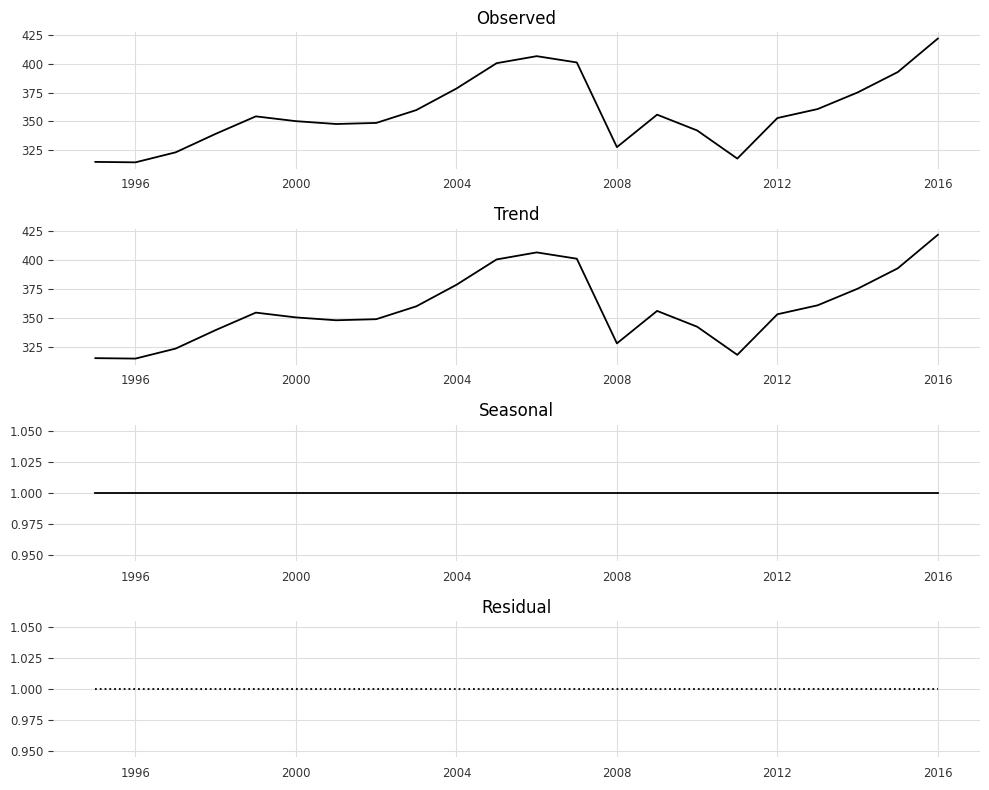
\includegraphics{hw3_files/figure-pdf/cell-23-output-1.png}

From the decomposition, it clear that there is minimal seasonality and
the trend line is unclear without further analysis. Thus, we believe
using Naive Mean forecast would be the best for this time series.

\begin{Shaded}
\begin{Highlighting}[]
\NormalTok{series }\OperatorTok{=}\NormalTok{ TimeSeries.from\_dataframe(aus\_wealth, value\_cols}\OperatorTok{=}\StringTok{\textquotesingle{}Wealth\textquotesingle{}}\NormalTok{)}

\NormalTok{model }\OperatorTok{=}\NormalTok{ NaiveMean()}

\NormalTok{model.fit(series)}

\NormalTok{forecast }\OperatorTok{=}\NormalTok{ model.predict(}\DecValTok{10}\NormalTok{)}

\NormalTok{series.plot()}
\NormalTok{forecast.plot(label}\OperatorTok{=}\StringTok{\textquotesingle{}NaiveMean Forecast\textquotesingle{}}\NormalTok{)}
\NormalTok{plt.legend()}
\end{Highlighting}
\end{Shaded}

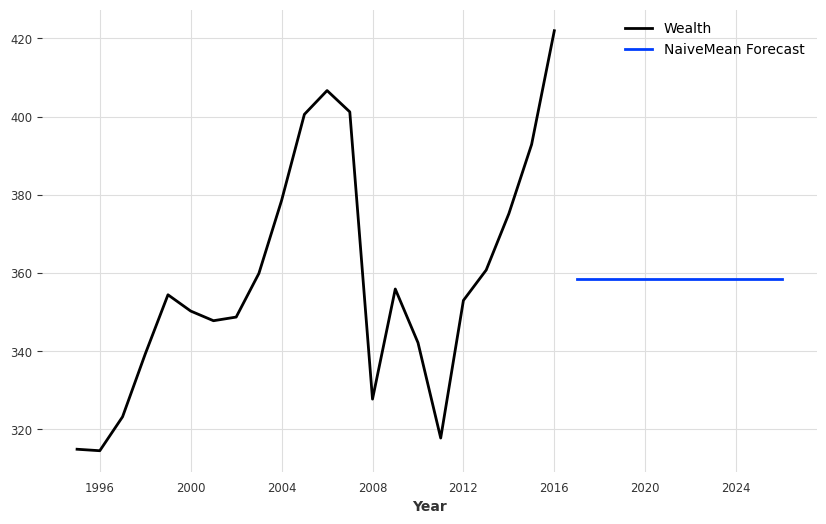
\includegraphics{hw3_files/figure-pdf/cell-24-output-1.png}

\subsubsection{\texorpdfstring{Australian takeaway food turnover from
\texttt{aus\_retail}}{Australian takeaway food turnover from aus\_retail}}\label{australian-takeaway-food-turnover-from-aus_retail}

We are going to filter take away food services in the Australian Capital
Territory because we tried plotting all of the territories in one plot
which leds to a overcrowded plot. Therefore, we will focus on the
Australian Capital Regions.

\begin{Shaded}
\begin{Highlighting}[]
\NormalTok{df\_takeaway }\OperatorTok{=}\NormalTok{ df\_retail.query(}\StringTok{\textquotesingle{}Industry == "Takeaway food services" \& State == "Australian Capital Territory"\textquotesingle{}}\NormalTok{)}
\NormalTok{df\_takeaway }\OperatorTok{=}\NormalTok{ df\_takeaway[[}\StringTok{\textquotesingle{}Month\textquotesingle{}}\NormalTok{, }\StringTok{\textquotesingle{}Turnover\textquotesingle{}}\NormalTok{]]}
\NormalTok{df\_takeaway.set\_index(}\StringTok{\textquotesingle{}Month\textquotesingle{}}\NormalTok{, inplace}\OperatorTok{=}\VariableTok{True}\NormalTok{)}
\end{Highlighting}
\end{Shaded}

\begin{Shaded}
\begin{Highlighting}[]
\NormalTok{df\_takeaway.plot()}
\NormalTok{plt.xlabel(}\StringTok{"Daily[1D]"}\NormalTok{)}
\NormalTok{plt.show()}
\end{Highlighting}
\end{Shaded}

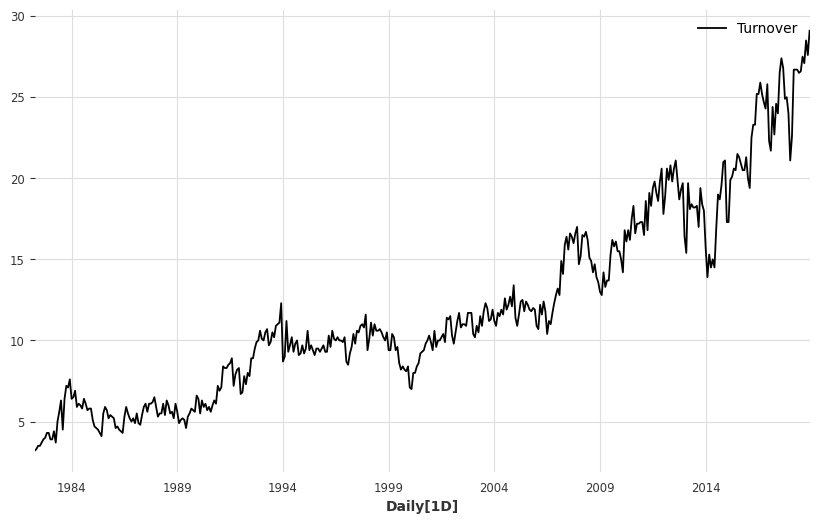
\includegraphics{hw3_files/figure-pdf/cell-26-output-1.png}

\begin{Shaded}
\begin{Highlighting}[]
\NormalTok{decomp }\OperatorTok{=}\NormalTok{ STL(df\_takeaway[}\StringTok{\textquotesingle{}Turnover\textquotesingle{}}\NormalTok{].values, period}\OperatorTok{=}\DecValTok{365}\NormalTok{).fit()}
\NormalTok{decomp.plot()}
\NormalTok{plt.show()}
\end{Highlighting}
\end{Shaded}

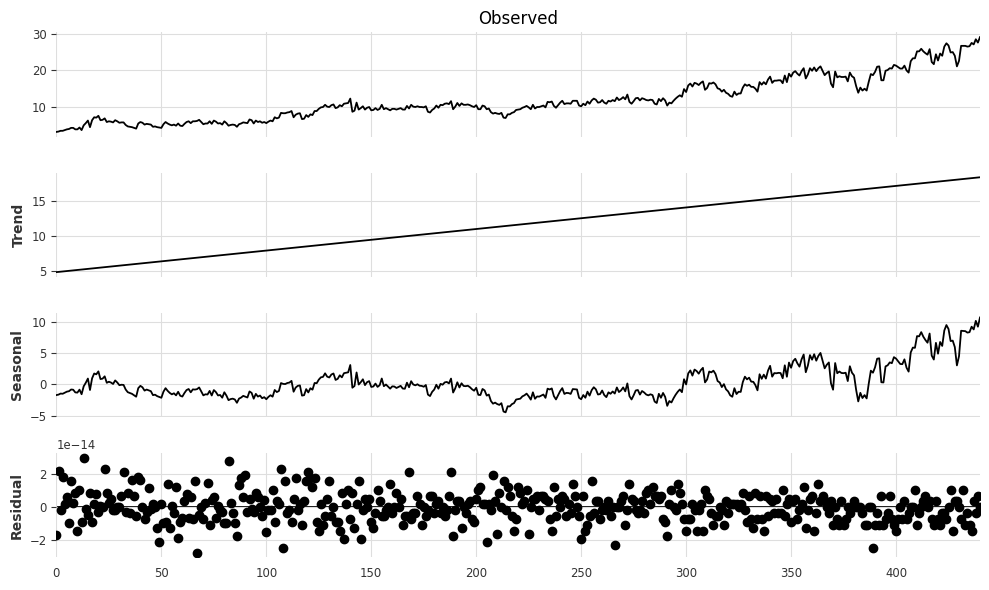
\includegraphics{hw3_files/figure-pdf/cell-27-output-1.png}

\begin{Shaded}
\begin{Highlighting}[]
\NormalTok{series }\OperatorTok{=}\NormalTok{ TimeSeries.from\_dataframe(df\_takeaway)}

\NormalTok{season\_model }\OperatorTok{=}\NormalTok{ NaiveSeasonal(K}\OperatorTok{=}\DecValTok{10}\NormalTok{) }\CommentTok{\# captures the pattern for 14 days (bi{-}weekly pattern)}
\NormalTok{drift\_model }\OperatorTok{=}\NormalTok{ NaiveDrift()}

\NormalTok{season\_model.fit(series)}
\NormalTok{drift\_model.fit(series)}

\NormalTok{seasonal\_forecast }\OperatorTok{=}\NormalTok{ season\_model.predict(}\DecValTok{60}\NormalTok{)}
\NormalTok{drift\_forecast }\OperatorTok{=}\NormalTok{ drift\_model.predict(}\DecValTok{60}\NormalTok{)}

\NormalTok{combined\_forecast }\OperatorTok{=}\NormalTok{ seasonal\_forecast }\OperatorTok{+}\NormalTok{ drift\_forecast }\OperatorTok{{-}}\NormalTok{ series.last\_value()}

\NormalTok{series.plot()}
\NormalTok{combined\_forecast.plot(label}\OperatorTok{=}\StringTok{\textquotesingle{}Combined (Drift and Seasonal Naive)\textquotesingle{}}\NormalTok{)}
\NormalTok{drift\_forecast.plot(label}\OperatorTok{=}\StringTok{\textquotesingle{}Drift\textquotesingle{}}\NormalTok{)}
\NormalTok{plt.legend()}
\NormalTok{plt.show()}
\end{Highlighting}
\end{Shaded}

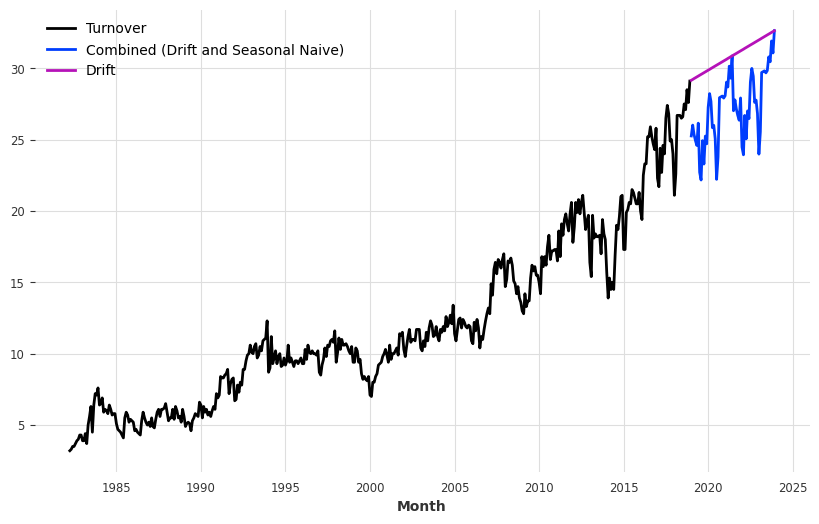
\includegraphics{hw3_files/figure-pdf/cell-28-output-1.png}

After decomposing the timeseries and observing that its overall trend is
increasing, we wanted to imploy a combination of the simple forecasting
methods. There is some seasonality but it was unclear the whether the
pattern was weeky or monthly. So, we decide to use bi-weekly to forcast
this timeseries.

\subsection{Exercise 2}\label{exercise-2}

Use the Facebook stock price (data set gafa\_stock) to do the following:

\begin{Shaded}
\begin{Highlighting}[]
\NormalTok{df\_gafa\_stock }\OperatorTok{=}\NormalTok{ pd.read\_csv(}\StringTok{"../rdata/gafa\_stock.csv"}\NormalTok{, parse\_dates }\OperatorTok{=}\NormalTok{ [}\StringTok{\textquotesingle{}Date\textquotesingle{}}\NormalTok{], index\_col }\OperatorTok{=}\NormalTok{ [}\StringTok{\textquotesingle{}Date\textquotesingle{}}\NormalTok{])}

\NormalTok{fb\_stock }\OperatorTok{=}\NormalTok{ df\_gafa\_stock.query(}\StringTok{\textquotesingle{}Symbol == "FB"\textquotesingle{}}\NormalTok{)}

\NormalTok{fb\_stock\_close }\OperatorTok{=}\NormalTok{ fb\_stock[}\StringTok{\textquotesingle{}Close\textquotesingle{}}\NormalTok{]}

\NormalTok{fb\_stock\_close }\OperatorTok{=}\NormalTok{ fb\_stock\_close.rename\_axis(}\StringTok{\textquotesingle{}Date\textquotesingle{}}\NormalTok{).reset\_index()}
\end{Highlighting}
\end{Shaded}

\begin{itemize}
\tightlist
\item
  Produce a time plot of the series.
\end{itemize}

\begin{Shaded}
\begin{Highlighting}[]
\NormalTok{fb\_stock\_close[}\StringTok{\textquotesingle{}Close\textquotesingle{}}\NormalTok{].plot(label}\OperatorTok{=}\StringTok{\textquotesingle{}Facebook Daily Closing Price\textquotesingle{}}\NormalTok{)}
\NormalTok{plt.legend()}
\NormalTok{plt.show()}
\end{Highlighting}
\end{Shaded}

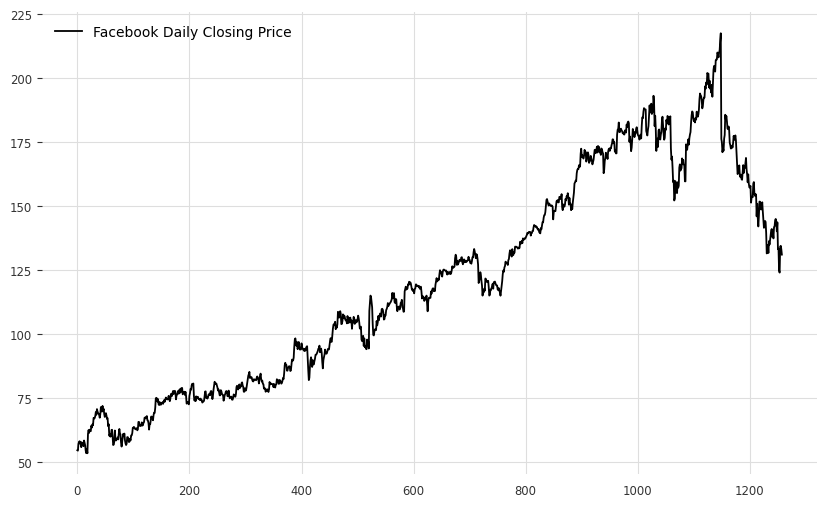
\includegraphics{hw3_files/figure-pdf/cell-30-output-1.png}

\begin{itemize}
\item
  Produce forecasts using the drift method and plot them.
\item
  Show that the forecasts are identical to extending the line drawn
  between the first and last observations.
\end{itemize}

For the next two bullet points, we will create a drift forecast of the
fb closing price data and then draw a dash line between the first and
last values to determine whether the drift forecast is identical to the
dash line.

\begin{Shaded}
\begin{Highlighting}[]

\NormalTok{series }\OperatorTok{=}\NormalTok{ TimeSeries.from\_dataframe(fb\_stock\_close, value\_cols}\OperatorTok{=}\StringTok{\textquotesingle{}Close\textquotesingle{}}\NormalTok{)}

\NormalTok{drift }\OperatorTok{=}\NormalTok{ NaiveDrift()}
\NormalTok{drift.fit(series)}

\NormalTok{forecast }\OperatorTok{=}\NormalTok{ drift.predict(}\DecValTok{100}\NormalTok{) }\CommentTok{\# predict the next 100 days since it is daily data}

\NormalTok{series.plot()}
\NormalTok{forecast.plot(label}\OperatorTok{=}\StringTok{\textquotesingle{}Drift Forecast\textquotesingle{}}\NormalTok{)}

\NormalTok{first\_value }\OperatorTok{=}\NormalTok{ series.first\_value()}
\NormalTok{last\_value }\OperatorTok{=}\NormalTok{ series.last\_value()}

\CommentTok{\# superimpose dash line on plot}
\NormalTok{plt.plot([series.time\_index[}\DecValTok{0}\NormalTok{], series.time\_index[}\OperatorTok{{-}}\DecValTok{1}\NormalTok{]], [first\_value, last\_value], }\StringTok{\textquotesingle{}{-}{-}\textquotesingle{}}\NormalTok{, color }\OperatorTok{=} \StringTok{\textquotesingle{}blue\textquotesingle{}}\NormalTok{)}

\NormalTok{plt.legend()}
\NormalTok{plt.show()}
\end{Highlighting}
\end{Shaded}

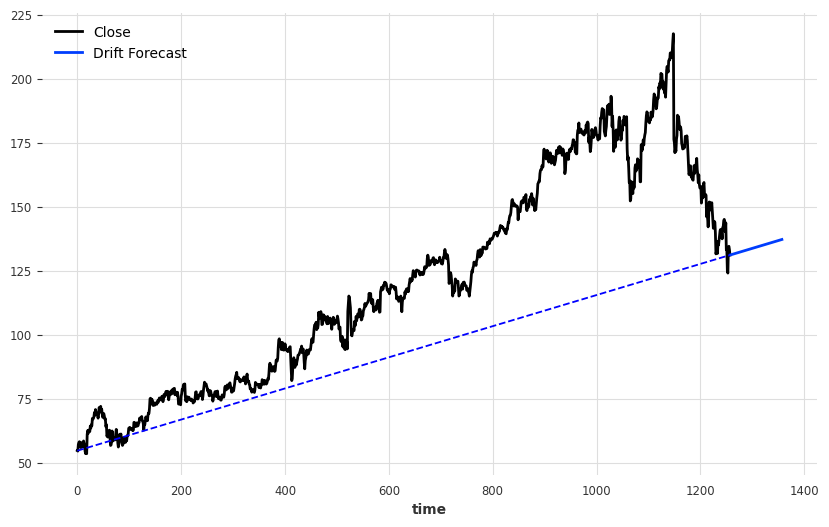
\includegraphics{hw3_files/figure-pdf/cell-31-output-1.png}

The drift forecast is identical to the superimposed dashed line on the
plot.

\begin{itemize}
\tightlist
\item
  Try using some of the other benchmark functions to forecast the same
  data set. Which do you think is best? Why?
\end{itemize}

We can observe that the drift method does not capture the seasonal
component of the data. So, we propose that a combination of NaiveSeaonal
and the drift method might be a better bencamrk function to forecast.

\begin{Shaded}
\begin{Highlighting}[]
\NormalTok{seasonal }\OperatorTok{=}\NormalTok{ NaiveSeasonal(K}\OperatorTok{=}\DecValTok{30}\NormalTok{)}
\NormalTok{seasonal.fit(series)}
\NormalTok{seasonal\_forecast }\OperatorTok{=}\NormalTok{ seasonal.predict(}\DecValTok{100}\NormalTok{)}
\NormalTok{combination }\OperatorTok{=}\NormalTok{ seasonal\_forecast }\OperatorTok{+}\NormalTok{ forecast }\OperatorTok{{-}}\NormalTok{ series.last\_value()}

\NormalTok{series.plot()}
\NormalTok{combination.plot(label}\OperatorTok{=}\StringTok{"Combined Drift and Naive Seasonal Forecast"}\NormalTok{)}
\NormalTok{plt.legend()}
\NormalTok{plt.show()}
\end{Highlighting}
\end{Shaded}

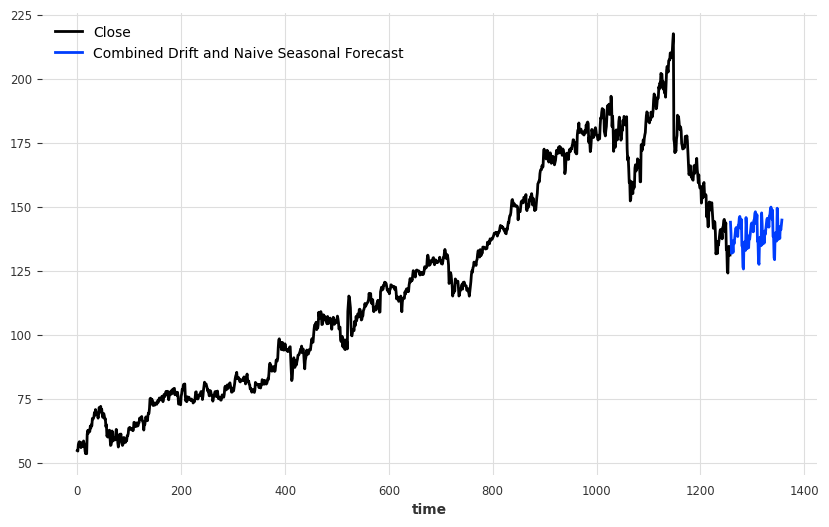
\includegraphics{hw3_files/figure-pdf/cell-32-output-1.png}

\subsection{Exercise 3}\label{exercise-3}

Apply a seasonal naïve method to the quarterly Australian beer
production data from 1992. Check if the residuals look like white noise,
and plot the forecasts. The following code will help.

\begin{Shaded}
\begin{Highlighting}[]
\NormalTok{\# Extract data of interest}
\NormalTok{recent\_production \textless{}{-} aus\_production |\textgreater{}}
\NormalTok{  filter(year(Quarter) \textgreater{}= 1992)}

\NormalTok{\# Define and estimate a model}
\NormalTok{fit \textless{}{-} recent\_production |\textgreater{} model(SNAIVE(Beer))}
\NormalTok{\#Look at the residuals}

\NormalTok{fit |\textgreater{} gg\_tsresiduals()}

\NormalTok{\# Look a some forecasts}
\NormalTok{fit |\textgreater{} forecast() |\textgreater{} autoplot(recent\_production)}
\end{Highlighting}
\end{Shaded}

What do you conclude?

\begin{Shaded}
\begin{Highlighting}[]
\NormalTok{aus\_beer }\OperatorTok{=}\NormalTok{ df\_production[[}\StringTok{\textquotesingle{}Quarter\textquotesingle{}}\NormalTok{, }\StringTok{\textquotesingle{}Beer\textquotesingle{}}\NormalTok{]]}
\NormalTok{aus\_beer }\OperatorTok{=}\NormalTok{ aus\_beer.query(}\StringTok{\textquotesingle{}Quarter \textgreater{}= "1992 Q1"\textquotesingle{}}\NormalTok{)}
\end{Highlighting}
\end{Shaded}

\begin{Shaded}
\begin{Highlighting}[]

\NormalTok{aus\_beer[}\StringTok{\textquotesingle{}Quarter\textquotesingle{}}\NormalTok{] }\OperatorTok{=}\NormalTok{ pd.to\_datetime(aus\_beer[}\StringTok{\textquotesingle{}Quarter\textquotesingle{}}\NormalTok{].astype(}\BuiltInTok{str}\NormalTok{), }\BuiltInTok{format} \OperatorTok{=} \StringTok{"\%Y Q\%m"}\NormalTok{)}
\NormalTok{aus\_beer}
\end{Highlighting}
\end{Shaded}

\begin{longtable}[]{@{}lll@{}}
\toprule\noalign{}
& Quarter & Beer \\
\midrule\noalign{}
\endhead
\bottomrule\noalign{}
\endlastfoot
144 & 1992-01-01 & 443 \\
145 & 1992-02-01 & 410 \\
146 & 1992-03-01 & 420 \\
147 & 1992-04-01 & 532 \\
148 & 1993-01-01 & 433 \\
... & ... & ... \\
213 & 2009-02-01 & 398 \\
214 & 2009-03-01 & 419 \\
215 & 2009-04-01 & 488 \\
216 & 2010-01-01 & 414 \\
217 & 2010-02-01 & 374 \\
\end{longtable}

\begin{Shaded}
\begin{Highlighting}[]
\NormalTok{aus\_beer.set\_index(}\StringTok{\textquotesingle{}Quarter\textquotesingle{}}\NormalTok{, inplace}\OperatorTok{=}\VariableTok{True}\NormalTok{)}
\end{Highlighting}
\end{Shaded}

\begin{verbatim}
KeyError: "None of ['Quarter'] are in the columns"
\end{verbatim}

\begin{Shaded}
\begin{Highlighting}[]

\NormalTok{aus\_beer}
\end{Highlighting}
\end{Shaded}

\begin{longtable}[]{@{}ll@{}}
\toprule\noalign{}
& Beer \\
Quarter & \\
\midrule\noalign{}
\endhead
\bottomrule\noalign{}
\endlastfoot
1992Q1 & 443 \\
1992Q1 & 410 \\
1992Q1 & 420 \\
1992Q2 & 532 \\
1993Q1 & 433 \\
... & ... \\
2009Q1 & 398 \\
2009Q1 & 419 \\
2009Q2 & 488 \\
2010Q1 & 414 \\
2010Q1 & 374 \\
\end{longtable}

\begin{Shaded}
\begin{Highlighting}[]
\NormalTok{aus\_beer.reset\_index(inplace}\OperatorTok{=}\VariableTok{True}\NormalTok{)}
\NormalTok{series }\OperatorTok{=}\NormalTok{ TimeSeries.from\_dataframe(aus\_beer, }\StringTok{\textquotesingle{}Quarter\textquotesingle{}}\NormalTok{, }\StringTok{\textquotesingle{}Beer\textquotesingle{}}\NormalTok{)}

\NormalTok{model }\OperatorTok{=}\NormalTok{ NaiveSeasonal(K}\OperatorTok{=}\DecValTok{4}\NormalTok{)}

\NormalTok{model.fit(series)}

\NormalTok{forecast }\OperatorTok{=}\NormalTok{ model.predict(}\DecValTok{4}\NormalTok{)}

\NormalTok{series.plot()}
\NormalTok{forecast.plot(label}\OperatorTok{=}\StringTok{\textquotesingle{}Naive Seasonal Forecast\textquotesingle{}}\NormalTok{)}
\NormalTok{plt.legend()}
\NormalTok{plt.show()}


\end{Highlighting}
\end{Shaded}

\begin{verbatim}
TypeError: Cannot interpret 'period[Q-DEC]' as a data type
\end{verbatim}

\subsection{Exercise 4}\label{exercise-4}

Repeat the previous exercise using the Australian Exports series from
global\_economy and the Bricks series from aus\_production. Use
whichever of NAIVE() or SNAIVE() is more appropriate in each case

\subsection{Exercise 7}\label{exercise-7}

For your retail time series (from Exercise 7 in Section 2.10):

\begin{enumerate}
\def\labelenumi{\alph{enumi}.}
\tightlist
\item
  Create a training dataset consisting of observations before 2011 using
\end{enumerate}

\begin{Shaded}
\begin{Highlighting}[]
\NormalTok{myseries\_train \textless{}{-} myseries |\textgreater{}}
\NormalTok{  filter(year(Month) \textless{} 2011)}
\end{Highlighting}
\end{Shaded}

\begin{enumerate}
\def\labelenumi{\alph{enumi}.}
\setcounter{enumi}{1}
\tightlist
\item
  Check that your data have been split appropriately by producing the
  following plot.
\end{enumerate}

\begin{Shaded}
\begin{Highlighting}[]
\NormalTok{autoplot(myseries, Turnover) +}
\NormalTok{  autolayer(myseries\_train, Turnover, colour = "red")}
\end{Highlighting}
\end{Shaded}

\begin{enumerate}
\def\labelenumi{\alph{enumi}.}
\setcounter{enumi}{2}
\tightlist
\item
  Fit a seasonal naïve model using SNAIVE() applied to your training
  data (myseries\_train).
\end{enumerate}

\begin{Shaded}
\begin{Highlighting}[]
\NormalTok{fit \textless{}{-} myseries\_train |\textgreater{}}
\NormalTok{  model(SNAIVE())}
\end{Highlighting}
\end{Shaded}

\begin{enumerate}
\def\labelenumi{\alph{enumi}.}
\setcounter{enumi}{3}
\tightlist
\item
  Check the residuals.
\end{enumerate}

\begin{Shaded}
\begin{Highlighting}[]
\NormalTok{fit |\textgreater{} gg\_tsresiduals()}
\end{Highlighting}
\end{Shaded}

Do the residuals appear to be uncorrelated and normally distributed?

e.Produce forecasts for the test data

\begin{Shaded}
\begin{Highlighting}[]
\NormalTok{fc \textless{}{-} fit |\textgreater{}}
\NormalTok{  forecast(new\_data = anti\_join(myseries, myseries\_train))}
\NormalTok{fc |\textgreater{} autoplot(myseries)}
\end{Highlighting}
\end{Shaded}

\begin{enumerate}
\def\labelenumi{\alph{enumi}.}
\setcounter{enumi}{5}
\tightlist
\item
  Compare the accuracy of your forecasts against the actual values.
\end{enumerate}

\begin{Shaded}
\begin{Highlighting}[]
\NormalTok{fit |\textgreater{} accuracy()}
\NormalTok{fc |\textgreater{} accuracy(myseries)}
\end{Highlighting}
\end{Shaded}

g.How sensitive are the accuracy measures to the amount of training data
used?



\end{document}
